\documentclass[a4paper,oneside,12pt]{amsart}

%\usepackage[spanish, activeacute]{babel}
\usepackage[utf8]{inputenc}
%\usepackage[latin1]{inputenc}
\usepackage{latexsym}
\usepackage{multicol}
\usepackage{enumerate}
\usepackage{enumitem}
\usepackage[heightrounded]{geometry}
\geometry{top=2cm,bottom=2cm,left=2cm,right=2cm}
\usepackage{graphicx}
\usepackage{tikz}
\usepackage{amssymb}
\usepackage{tikz-network}

\DeclareMathOperator{\cond}{cond}
\DeclareMathOperator{\Id}{Id}
\DeclareMathOperator{\re}{Re}
%\DeclareMathOperator{\im}{Im}
\newcommand{\I}{\mathbb{I}}
\newcommand{\R}{\mathbb{R}}
\newcommand{\Q}{\mathbb{Q}}
\newcommand{\C}{\mathbb{C}}
\newcommand{\Z}{\mathbb{Z}}
\newcommand{\N}{\mathbb{N}}
\DeclareMathOperator{\im}{Im}

\newcommand{\nombremateria}
{Investigaci\'on Operativa}
\newcommand{\nombrecuatrimestre}
    {Segundo cuatrimestre de 2021}
\newcommand{\numeroparcial}
    {Recuperatorio del Tercer Parcial }
\newcommand{\fecha}
    {10 de Diciembre de 2021}
\newcommand{\numerotema}
    {\bf 1}

%\oddsidemargin -1cm \evensidemargin -1cm \textwidth 17.5cm
%topmargin 1.2cm \textheight 25cm
%\setlength{\textheight}{25cm}

\def \ds{\displaystyle}
\newtheorem{quest}{Ejercicio}
\thispagestyle{empty}

\begin{document}

\hfill \hfill
\begin{tabular}[c]{|c|c|c|c|c|c|}
\hline 
1 & 2 & 3 & 4 & 5 & Calificaci\'on \\ \hline \hline
\hspace{1.2 cm} & \hspace{1.2 cm} & \hspace{1.2 cm} & \hspace{1.2 cm} & \hspace{1.2 cm} &\hspace{1.5 cm} \\
\hspace{1.2 cm} & \hspace{1.2 cm} & \hspace{1.2 cm} & \hspace{1.2 cm} & \hspace{1.2 cm} &\hspace{1.5 cm} \\ \hline

\end{tabular}

\vspace{-1cm}

\noindent Nombre y apellido:

\vspace{0.2cm}

\noindent Número de libreta:

\noindent \hrulefill 

\smallskip
\renewcommand{\baselinestretch}{1.1}

\begin{center}
	\large \textbf{\nombremateria} 
	
	\numeroparcial -- \fecha
\end{center}

\vspace{.6cm}
\renewcommand{\theenumi}{\textbf{\arabic{enumi}}}

%%% EMPIEZA EL EJERCICIO 1 %%%

\begin{quest} 
Sea $\mathcal{G}$ un grafo conexo y pesado, cuyas aristas no necesariamente tienen todos pesos distintos. Mostrar que si para toda partición de $\mathbb{V}$ en dos conjuntos disjuntos $\mathbb{V}_1$, $\mathbb{V}_2$ existe una única arista de peso mínimo que los conecta, entonces el AGM de $\mathcal{G}$ es único.

\end{quest}

%%% TERMINA EL EJERCICIO 1 %%%

%%% EMPIEZA EL EJERCICIO 2 %%%

\begin{quest} \hfill
\begin{enumerate} 
    \item Se dice que un grafo $G$ es biconexo si no tiene puntos de corte. Mostrar que si:
    \begin{enumerate}[label=\alph*)]
        \item $G$ no es biconexo, o
        \item $G$ es bipartito con bipartición $(V_1, V_2)$ tal que $|V_1|\neq|V_2|$
    \end{enumerate}
    entonces $G$ no tiene circuito hamiltoniano.

    \item Se tiene la siguiente red $G$ por la que pasa cierto flujo $f$. La red cuenta con dos fuentes $s_1, s_2$ y un sumidero $t$. Plantear el problema como un problema al cual pueda aplicársele un algoritmo de tipo Ford-Fulkerson para hallar flujo máximo y utilizar dicho algoritmo para resolverlo, considerando a $f$ como flujo inicial.
    
    \begin{center}
        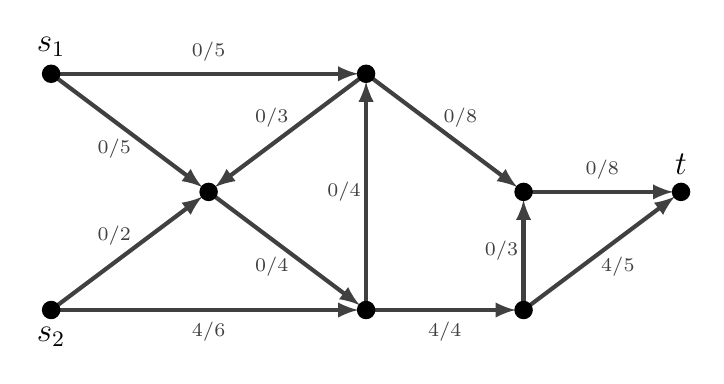
\begin{tikzpicture}
            \SetVertexStyle[FillColor=black, MinSize=0.7]
            \Vertex[label=$s_1$, position=above, fontsize=\large, x=0, y=1.5]{s1}
            \Vertex[label=$s_2$, position=below, fontsize=\large, x=0, y=-1.5]{s2}
            \Vertex[x=2, y=0]{u1}
            \Vertex[x=4, y=1.5]{u2}
            \Vertex[x=4, y=-1.5]{u3}
            \Vertex[x=6, y=0]{u4}
            \Vertex[x=6, y=-1.5]{u5}
            \Vertex[label=$t$, position=above, x=8, y=0, fontsize=\large]{t}
            \Edge[Direct, label=$0/5$, position=below left](s1)(u1)
            \Edge[Direct, label=$0/2$, position=above left](s2)(u1)
            \Edge[Direct, label=$0/5$, position=above](s1)(u2)
            \Edge[Direct, label=$4/6$, position=below](s2)(u3)
            \Edge[Direct, label=$0/3$, position=above left](u2)(u1)
            \Edge[Direct, label=$0/4$, position=below left](u1)(u3)
            \Edge[Direct, label=$0/4$, position=left](u3)(u2)
            \Edge[Direct, label=$0/8$, position=above right, distance=0.5](u2)(u4)
            \Edge[Direct, label=$4/4$, position=below](u3)(u5)
            \Edge[Direct, label=$0/3$, position=left](u5)(u4)
            \Edge[Direct, label=$0/8$, position=above](u4)(t)
            \Edge[Direct, label=$4/5$, position=below right](u5)(t)
            
        \end{tikzpicture}
    \end{center}
\end{enumerate}
\end{quest}

%%% TERMINA EL EJERCICIO 2 %%%

%%% EMPIEZA EL EJERCICIO 3 %%%


\begin{quest} 
Calcular la cantidad de formas de colorear las cliques maximales con a lo sumo $k$ colores del siguiente grafo de forma tal que a cliques maximales que tengan vértices en común se les asignen colores distintos. Modelar el problema y resolver utilizando alguno de los algoritmos vistos en la materia. 

\begin{figure}[h]
    \centering
    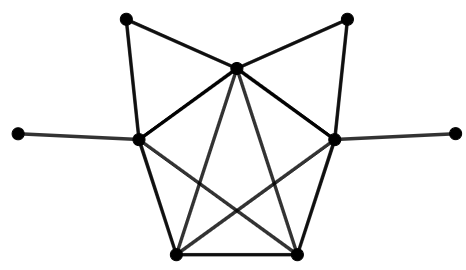
\includegraphics[width=8cm]{Imagenes/Ej3-RP1-IO2021.PNG}
\end{figure}
 
\end{quest}

%%% TERMINA EL EJERCICIO 3 %%%

%%% EMPIEZA EL EJERCICIO 4 %%%

\begin{quest} 
Un grafo se dice "arco-circular" si es el grafo intersección de arcos abiertos alrededor de un círculo, es decir, si se pueden representar sus vértices a través de dichos arcos de modo de que cada intervalo está asociado a un vértice y dos vertices son adyacentes si y solo si los arcos se intersectan. Por ejemplo el siguiente grafo: 
\begin{center}
    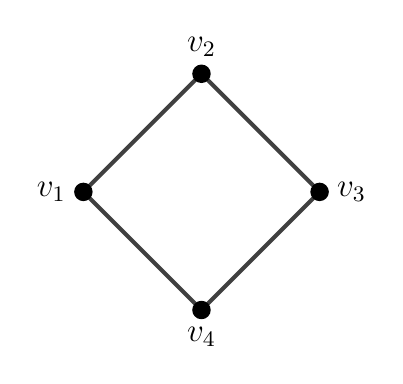
\begin{tikzpicture}
        \SetVertexStyle[FillColor=black, MinSize=0.7]
        \Vertex[label=$v_1$, position=left, fontsize=\large, x=0, y=0]{v1}
        \Vertex[label=$v_2$, position=above, fontsize=\large, x=1.5, y=1.5]{v2}
        \Vertex[label=$v_3$, position=right, fontsize=\large, x=3, y=0]{v3}
        \Vertex[label=$v_4$, position=below, fontsize=\large, x=1.5, y=-1.5]{v4}
        \Edge(v1)(v2)
        \Edge(v2)(v3)
        \Edge(v3)(v4)
        \Edge(v4)(v1)
    \end{tikzpicture}
\end{center}
es arco-circular porque tiene, entre otras, la siguiente representación en arcos:

\begin{center}
    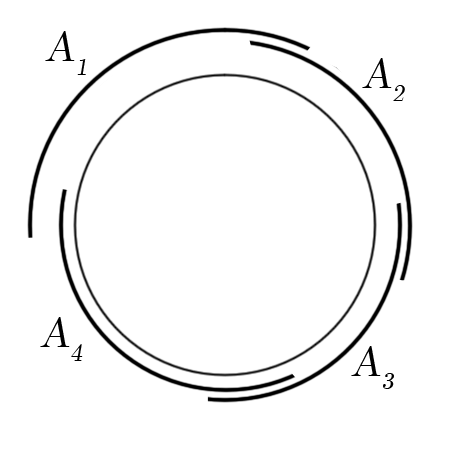
\includegraphics[scale=1.3]{Imagenes/arc.png}
\end{center}
% (dibujar A_1 que se interseque con A_2, A_2 con A_3. A_3 con A_4 y A_4 con A_1) 

\begin{enumerate}[label=\alph*)]
    \item Mostrar un grafo que no sea arco-circular. Justificar.
    \item Un grafo arco-circular es arco-circular-unitario, si existe una representación de modo que todos los arcos tengan la misma longitud. Mostrar que el siguiente grafo: 
    \begin{center}
        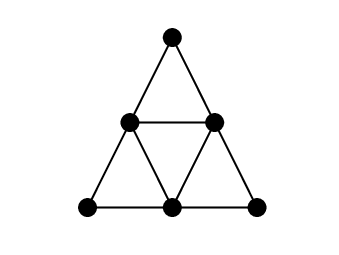
\includegraphics[]{Imagenes/The-Hajos-Graph.png}
        % \begin{tikzpicture}
        %     \SetVertexStyle[FillColor=black, MinSize=0.7]
        %     \Vertex[x=0, y=0]{v1}
        %     \Vertex[x=4, y=0]{v2}
        %     \Vertex[x=2, y=1.3]{v3}
        %     \Vertex[x=2, y=3]{v4}
        %     \Edge(v1)(v2)
        %     \Edge(v2)(v3)
        %     \Edge(v2)(v4)
        %     \Edge(v3)(v4)
        %     \Edge(v1)(v4)
        %     \Edge(v1)(v3)
        % \end{tikzpicture}
    \end{center}
    es arco-circular pero NO es arco-circular-unitario.
\end{enumerate}
\end{quest}

%%% TERMINA EL EJERCICIO 4 %%%

%%% EMPIEZA EL EJERCICIO 5 %%%

\begin{quest}

Dada una matriz binaria $A\in\{0,1\}^{n\times m}$, el $0$ representa agua y el $1$ representa tierra.  Decimos que un conjunto maximal de $1$'s adyacentes forman una isla (ver ejemplo). Modelar como un problema de grafos y proponer un algoritmo que permita resolver el problema de contar la cantidad de islas en tiempo polinomial.

Por ejemplo, dada la matriz:
\[
A = \begin{pmatrix}
1 & 0 & 1 & 0 & 0  & 0 & 1 & 1 & 1 & 1 \\
0 & 0  & 1 & 0 & 1  & 0 & 1 & 0 & 0 & 0 \\
1 & 1  & 1 & 1 & 0  & 0 & 1 & 0 & 0 & 0 \\
1 & 0  & 0 & 1 & 0  & 1 & 0 & 0 & 0 & 0 \\
1 & 1  & 1 & 1 & 0  & 0 & 0 & 1 & 1 & 1 \\
0 & 1  & 0 & 1 & 0  & 0 & 1 & 1 & 1 & 1 \\
0 & 0  & 0 & 0 & 0  & 1 & 1 & 1 & 0 & 0 \\
0 & 0  & 0 & 1 & 0  & 0 & 1 & 1 & 1 & 0 \\
1 & 0  & 1 & 0 & 1  & 0 & 0 & 1 & 0 & 0 \\
1 & 1  & 1 & 1 & 0  & 0 & 0 & 1 & 1 & 1 \\
\end{pmatrix}
\]
Tenemos $5$ islas:

\begin{center}
    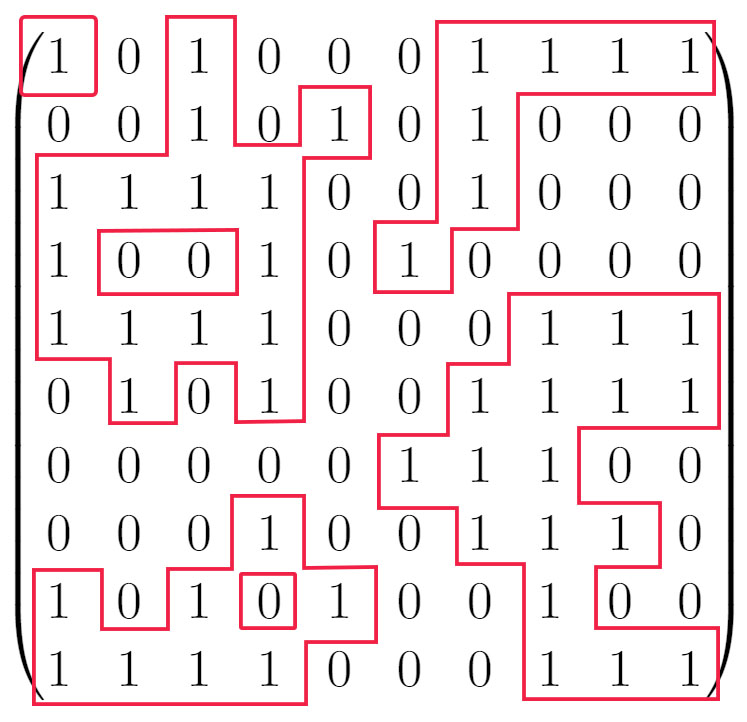
\includegraphics[scale=0.24]{Imagenes/parcial.jpg}
\end{center}

\end{quest}

%%% TERMINA EL EJERCICIO 5 %%%

%%% TERMINA EL PARCIAL %%%



\end{document}

